\section{Analisi di Fourier}
L'analisi di Fourier decompone il segnale in costituenti sinusoidali di differenti frequenze. Il segnale non è più nel dominio tempo-spazio, ma delle frequenze: i dati sono gli stessi, cambia solo la rappresentazione.

\textit{Ogni funzione periodica e a quadrato sommabile può essere espressa come somma di funzioni seno e coseno (combinazioni di funzioni armoniche).}

Si ricorda che una sequenza periodica è $x(n) = x(n + T)$. Una funzione armonica è una funzione periodica del tipo:
$$y = A\sin(\varpi x + \varphi) \qquad y = A\cos(\varpi x + \varphi)$$
Dove $A$ è l'ampiezza, $\varpi$ è la pulsazione, $\varphi$ è la fase. Si ha che $\varpi = 2\pi/T$ dove $1/T$ è la frequenza, e $\pi$ è $180^{\circ}$.

Sviluppando i seni e i coseni si ha, con $a = A\sin(\varphi)$ e $b = A\cos(\varphi)$: \\
$y = A\sin(\varpi x + \varphi) = a\cos (\varpi x) + b\sin(\varpi x)$ \\
$y = A\cos(\varpi x + \varphi) = b\cos(\varpi x) + a\sin(\varpi x)$ \\

Le armoniche vengono combinate una per volta, avvicinandosi man mano alla funzione originaria.
\begin{figure}[h]
	\centering
	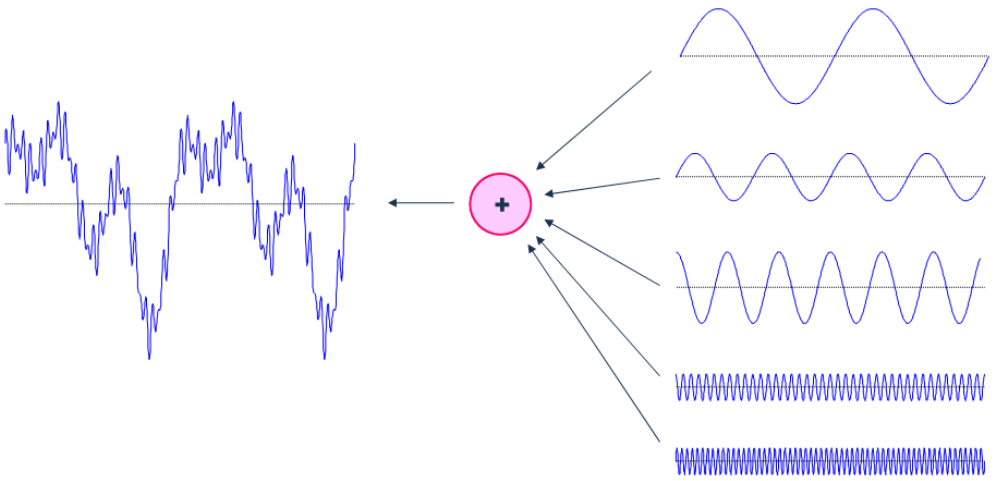
\includegraphics[scale=0.43]{Lezioni/Immagini/fourier}
\end{figure}

\subsection{Serie di Fourier}
La serie di Fourier è una formula utile per approssimare la scomposizione. Rappresenta una funzione periodica mediante combinazione lineare di funzioni sinusoidali.
$$f(x) = \frac{a_0}{2} + \sum_{k=1}^{\infty} a_k \cos\Big(\frac{2\pi}{N}kx\Big) + b_k\sin\Big(\frac{2\pi}{N}kx\Big)$$
$$N \rightarrow \text{periodo} \qquad (1/N) \rightarrow \text{frequenza fondamentale } f_0 \qquad (1/N)k \rightarrow \text{frequenze multiple } kf_0$$

$a_k$ e $b_k$ sono numeri reali, $k$ è un numero intero che funge da fattore moltiplicativo e $N$ è l'ampiezza della parte di funzione che si ripete periodicamente.

Con tempo $T = 1/f$ il dominio del tempo è $t$, e il dominio della frequenza è $Hz$.

Estendendo la formula con il concetto di pulsazione, si ha che una pulsazione è $\varpi_k = 2\pi f_k$, e di conseguenza:
$$f(x) = \frac{a_0}{2} + \sum_{k=1}^{\infty} a_k \cos(2\pi kf_0x) + b_k\sin(2\pi kf_0x)$$
$$a_k = \frac{2}{N} \int_{-\frac{N}{2}}^{\frac{N}{2}} f(x)\cos(2\pi kf_0x) dx \qquad b_k = \frac{2}{N} \int_{-\frac{N}{2}}^{\frac{N}{2}} f(x)\sin(2\pi kf_0x) dx$$

Si ricorda che $N$ è il periodo. Data la funzione $f(x)$ periodica, i coefficienti della serie sono \textbf{univocamente} determinati. I coefficienti sono i fattori moltiplicativi di seno e coseno, in relazione al tempo $t$.

\subsection{Fourier e i suoni}
I suoni elementari hanno andamento sinusoidale, periodico e con estensione indefinita; la maggior parte dei suoni in natura sono però caratterizzati da forme d'onda diverse.

Si può dimostrare che, fatte alcune ipotesi di regolarità sull'andamento della forma d'onda, un generico suono complesso può essere descritto come una combinazione di suoni elementari (armoniche).








